\chapter{结果展示}
下面我们展示我们的算法和原在一些例子上一些结果,并与原算法做一个比较,说明我们的算法的优势。我们定义误差$\delta$为该三角网格的外接球的直径的百分比。从结果中我们可以发现,我们的形变算法能够根据原网格的各项异性信息,有效地将原网格形变成为一个更趋于各项同性的网格,从而在形变之后的网格上的3D Delaunay三角化对应于原网格上则是带有其各项异性信息的三角化方法,从而优化了细化的结果,不仅减少了后序的简化操作,而且优化了简化结果。所有的实验结果均在一台CPU为Interlxxx,内存为XXX的机器上运行得到。

\section{Cylinder模型}
在一个细长的圆柱体模型(顶点数量为10000)上,我们的算法和原算法的结果对比:
\begin{figure}[htbp]
  \centering
  \begin{subfigure}[b]{0.4\textwidth}
    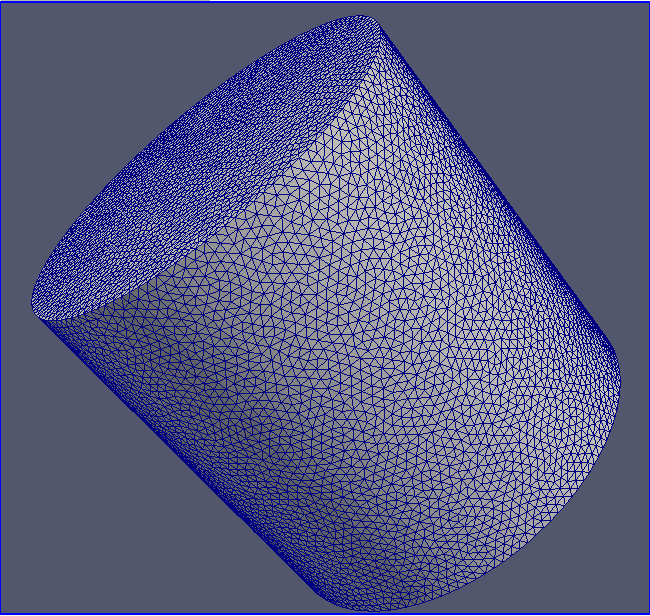
\includegraphics[width=\textwidth]{cylinder.png}
    \end{subfigure}
    \begin{subfigure}[b]{0.4\textwidth}
      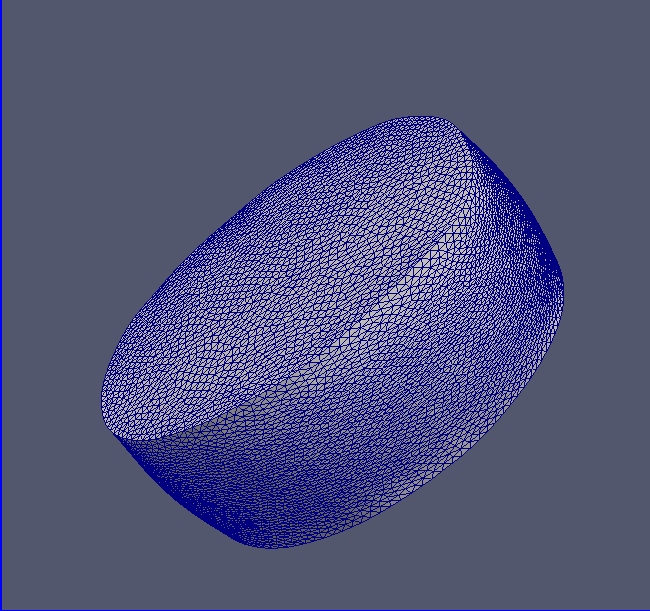
\includegraphics[width=\textwidth]{cylinder_deformed.png}
    \end{subfigure}
    \caption[Cylinder形变结果]{原网格(a)和用我们的形变算法形变之后的网格(b)}
    \label{fig:cylinder-deform}
\end{figure}


\begin{figure}[htbp]
  \centering
  \begin{subfigure}[b]{0.4\textwidth}
    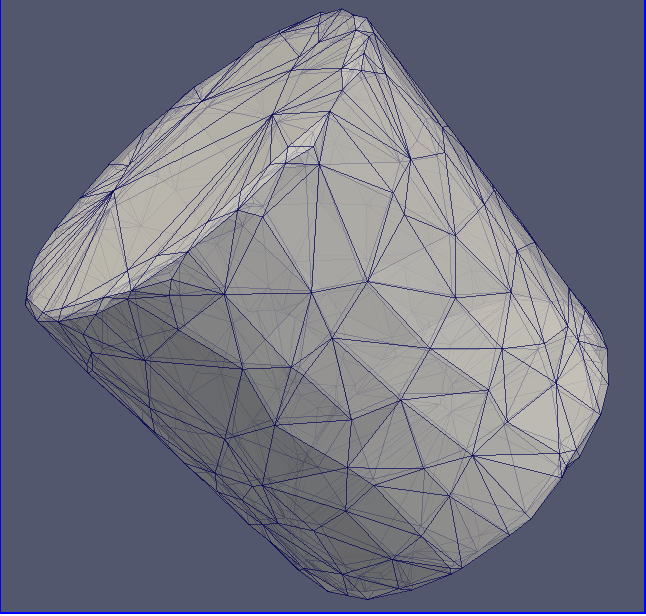
\includegraphics[width=\textwidth]{CYLINDER_0_0.02_0.02_0.04_100_refine.png}
  \end{subfigure}
  \begin{subfigure}[b]{0.4\textwidth}
    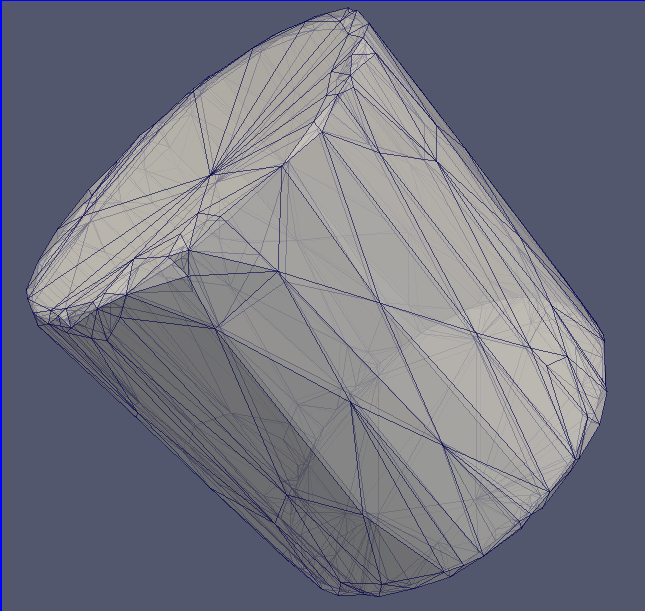
\includegraphics[width=\textwidth]{CYLINDER_1_0.02_0.02_0.04_100_refine.png}
  \end{subfigure}
  \begin{subfigure}[b]{0.4\textwidth}
    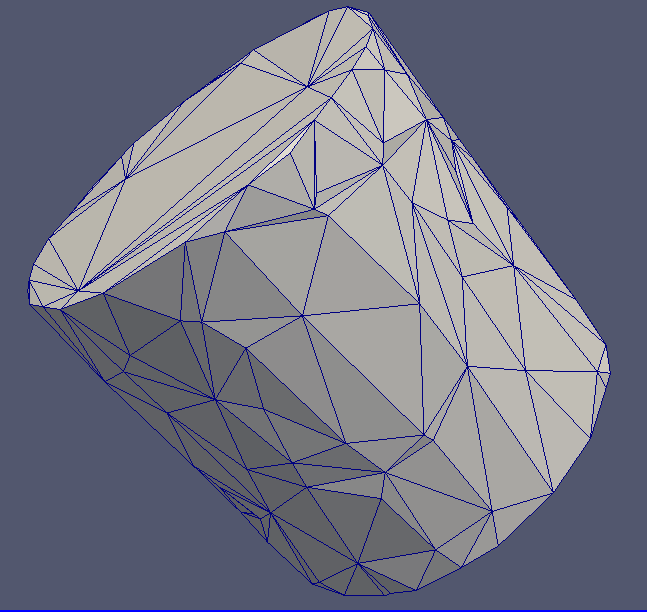
\includegraphics[width=\textwidth]{CYLINDER_0_0.02_0.02_0.04_100.png}
  \end{subfigure}
  \begin{subfigure}[b]{0.4\textwidth}
    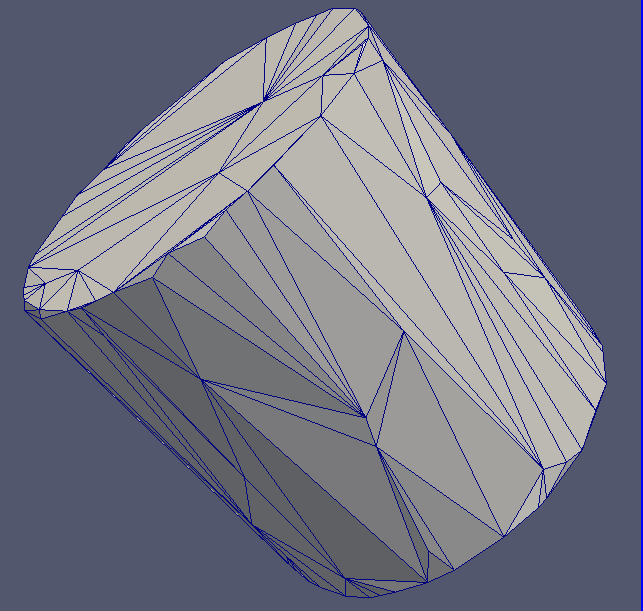
\includegraphics[width=\textwidth]{CYLINDER_1_0.02_0.02_0.04_100.png}
  \end{subfigure}
  \caption[当$\delta=0.58\%$时Cylinder结果对比]{当$\delta=0.58\%$时,原算法的细化结果(左上图)和我们的算法的细化结果(右上图),原算法的简化结果(左下图,最终顶点数量为192)和我们的算法的简化结果(右下图,最终顶点数量为132)}
  \label{fig:cylinder-res1}
\end{figure}

\begin{figure}[htbp]
  \centering
  \begin{subfigure}[b]{0.4\textwidth}
    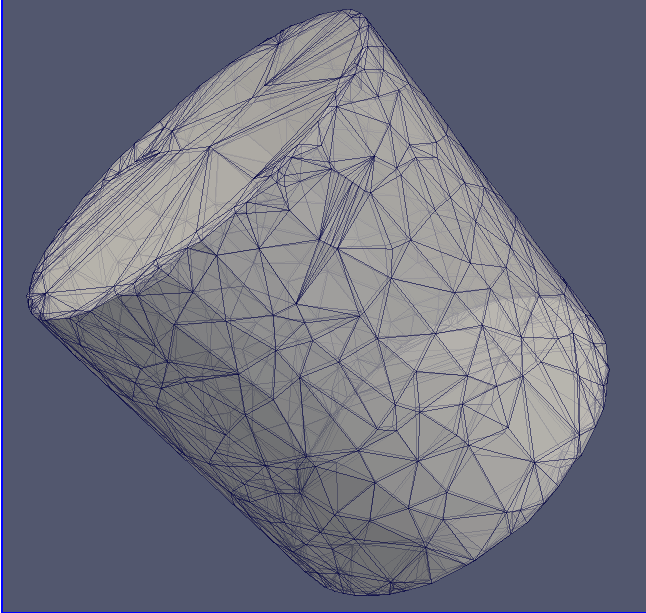
\includegraphics[width=\textwidth]{CYLINDER_0_0.01_0.005_0.02_100_refine.png}
  \end{subfigure}
  \begin{subfigure}[b]{0.4\textwidth}
    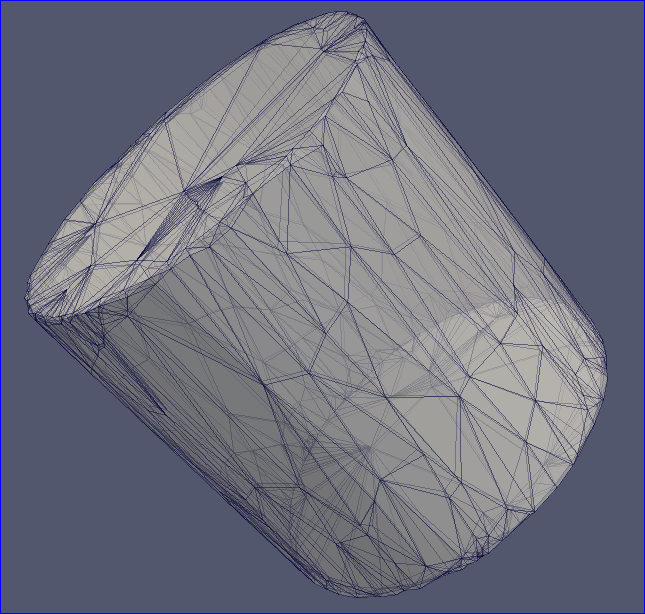
\includegraphics[width=\textwidth]{CYLINDER_1_0.01_0.005_0.02_100_refine.png}
  \end{subfigure}
  \begin{subfigure}[b]{0.4\textwidth}
    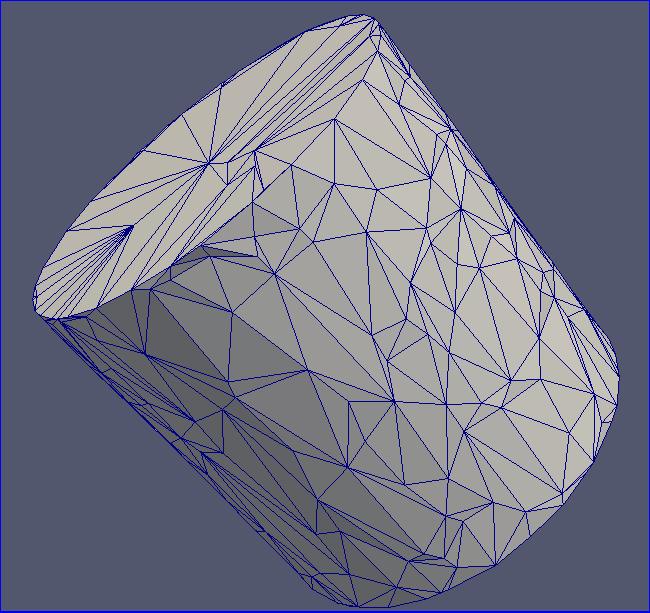
\includegraphics[width=\textwidth]{CYLINDER_0_0.01_0.005_0.02_100.png}
  \end{subfigure}
  \begin{subfigure}[b]{0.4\textwidth}
    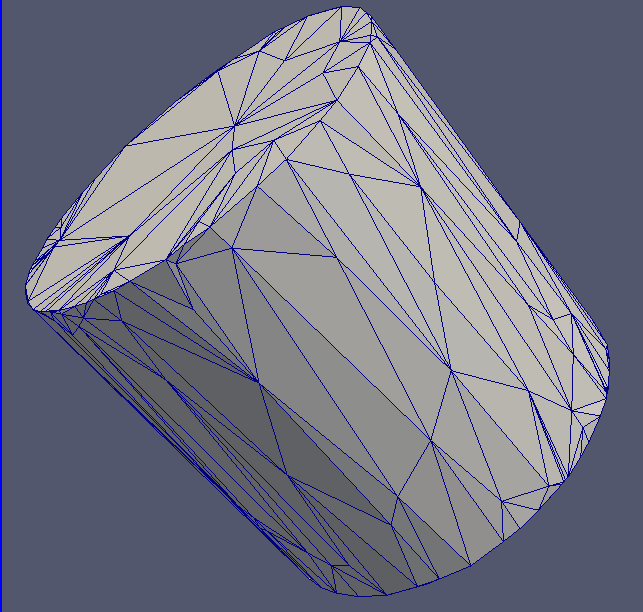
\includegraphics[width=\textwidth]{CYLINDER_1_0.01_0.005_0.02_100.png}
  \end{subfigure}
  \caption[当$\delta=0.29\%$时Cylinder结果对比]{当$\delta=0.29\%$时,原算法的细化结果(左上图)和我们的算法的细化结果(右上图),原算法的简化结果(左下图,最终顶点数量为350)和我们的算法的简化结果(右下图,最终顶点数量为254)}
  \label{fig:cylinder-res2}
\end{figure}

%% 原网格 - 形变之后的网格
%% \delta=? 时的对比
%% \delta=? 时的对比
%% \delta=? 时时间和顶点数量列表和原来算法的对比

\section{Cigar模型}
在一个细长的雪茄体模型(顶点数量为5000)上,我们的算法和原算法的结果对比:
\begin{figure}[htbp]
  \centering
  \begin{subfigure}[b]{0.4\textwidth}
    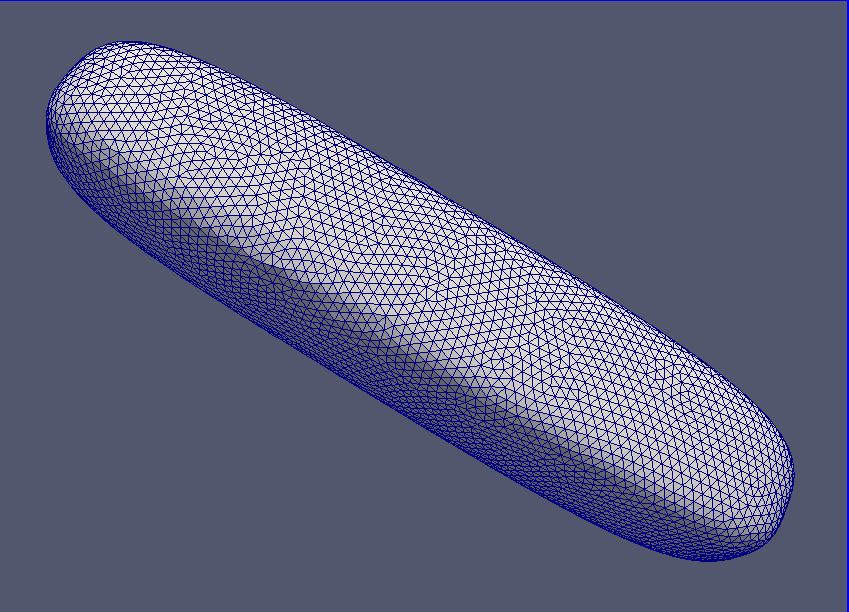
\includegraphics[width=\textwidth]{cigar.png}
    \end{subfigure}
    \begin{subfigure}[b]{0.4\textwidth}
      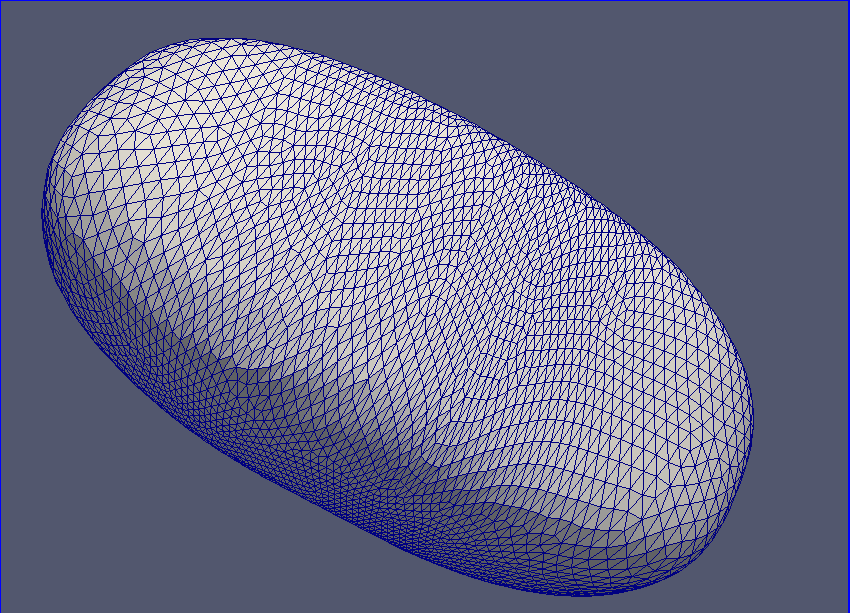
\includegraphics[width=\textwidth]{cigar_deformed.png}
    \end{subfigure}
    \caption[cigar形变结果]{原网格(a)和用我们的形变算法形变之后的网格(b)}
    \label{fig:cigar-deform}
\end{figure}


\begin{figure}[htbp]
  \centering
  \begin{subfigure}[b]{0.4\textwidth}
    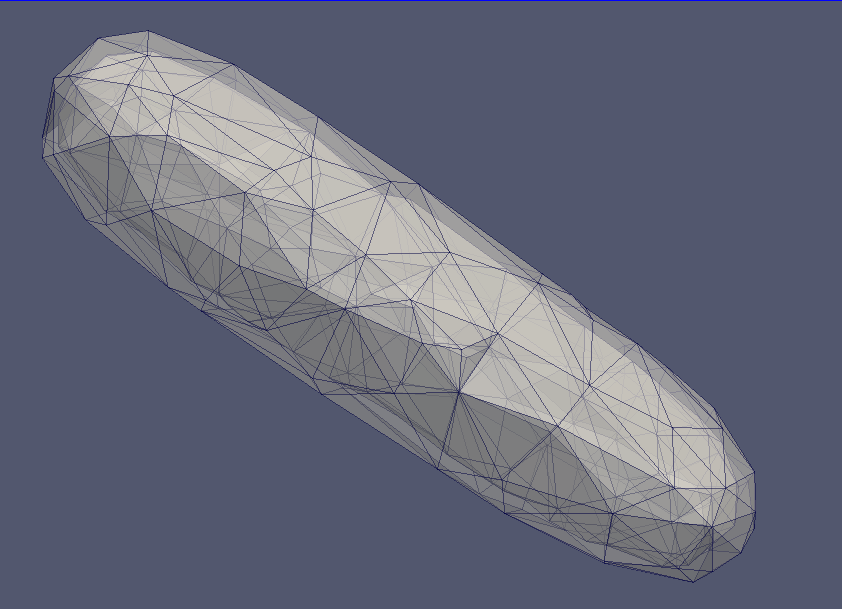
\includegraphics[width=\textwidth]{CIGAR_0_0.1_0.05_0.1_100_refine.png}
  \end{subfigure}
  \begin{subfigure}[b]{0.4\textwidth}
    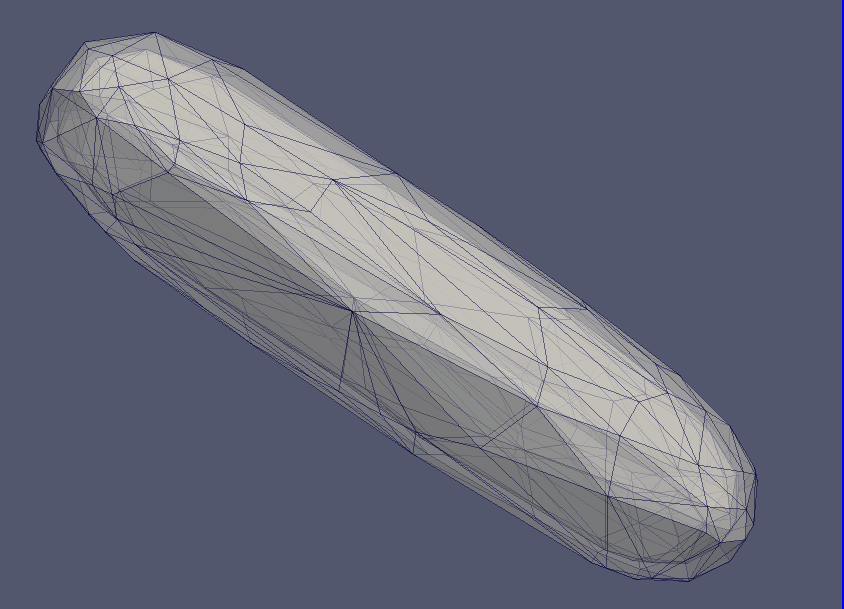
\includegraphics[width=\textwidth]{CIGAR_1_0.1_0.05_0.1_100_refine.png}
  \end{subfigure}
  \begin{subfigure}[b]{0.4\textwidth}
    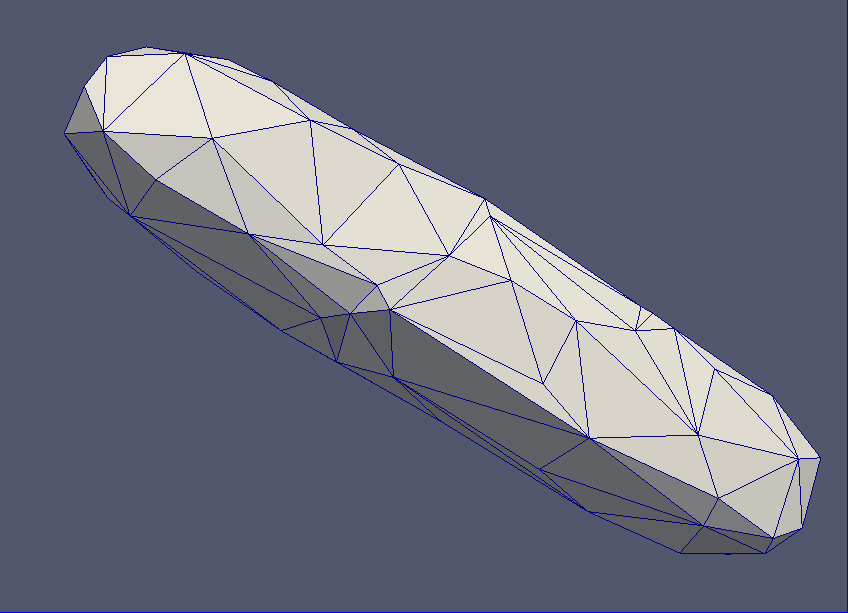
\includegraphics[width=\textwidth]{CIGAR_0_0.1_0.05_0.1_100.png}
  \end{subfigure}
  \begin{subfigure}[b]{0.4\textwidth}
    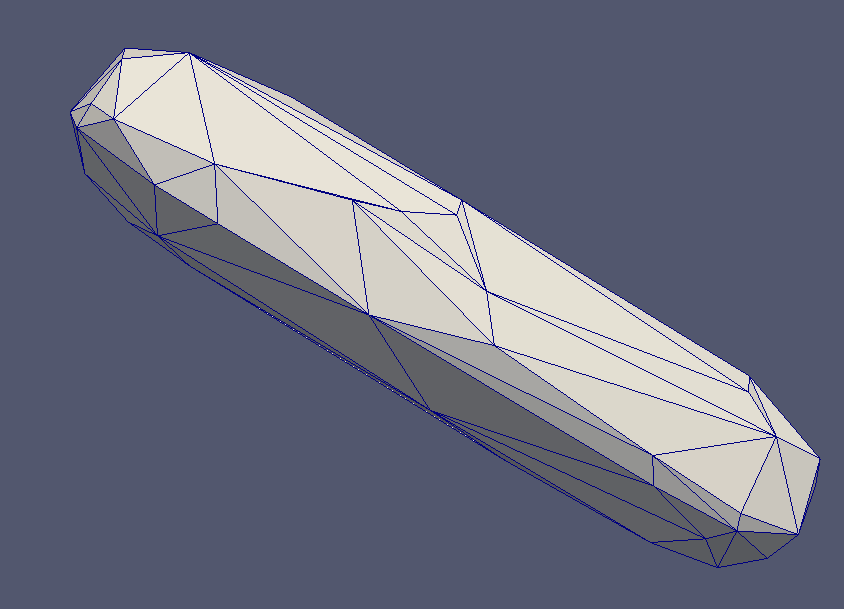
\includegraphics[width=\textwidth]{CIGAR_1_0.1_0.05_0.1_100.png}
  \end{subfigure}
  \caption[当$\delta=1.06\%$时cigar结果对比]{当$\delta=1.06\%$时,原算法的细化结果(左上图)和我们的算法的细化结果(右上图),原算法的简化结果(左下图,最终顶点数量为89)和我们的算法的简化结果(右下图,最终顶点数量为69)}
  \label{fig:cigar-res1}
\end{figure}

\begin{figure}[htbp]
  \centering
  \begin{subfigure}[b]{0.4\textwidth}
    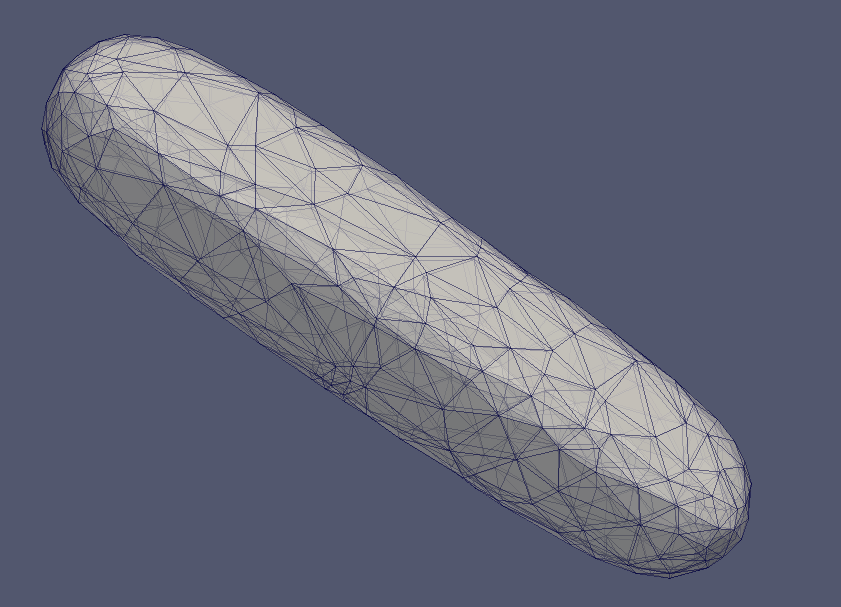
\includegraphics[width=\textwidth]{CIGAR_0_0.03_0.015_0.03_100_refine.png}
  \end{subfigure}
  \begin{subfigure}[b]{0.4\textwidth}
    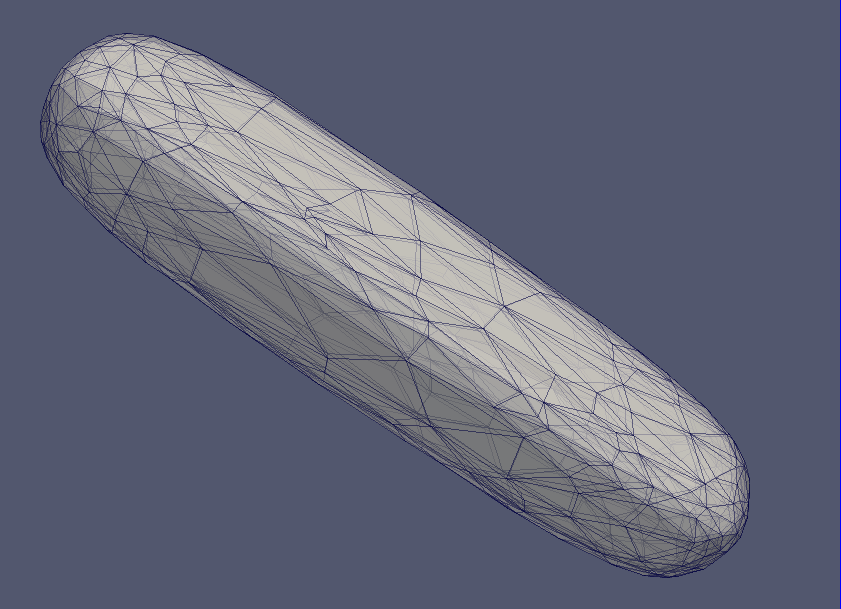
\includegraphics[width=\textwidth]{CIGAR_1_0.03_0.015_0.03_100_refine.png}
  \end{subfigure}
  \begin{subfigure}[b]{0.4\textwidth}
    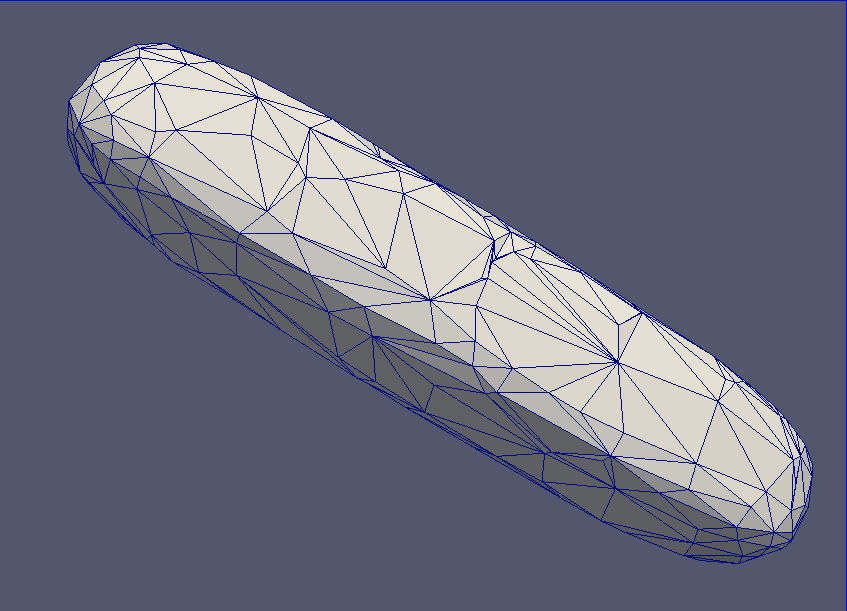
\includegraphics[width=\textwidth]{CIGAR_0_0.03_0.015_0.03_100.png}
  \end{subfigure}
  \begin{subfigure}[b]{0.4\textwidth}
    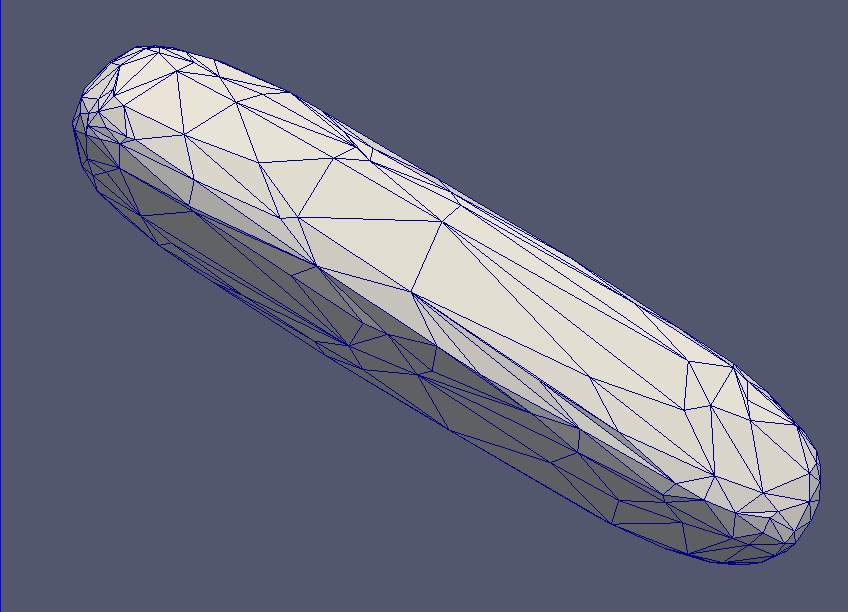
\includegraphics[width=\textwidth]{CIGAR_1_0.03_0.015_0.03_100.png}
  \end{subfigure}
  \caption[当$\delta=0.32\%$时cigar结果对比]{当$\delta=0.32\%$时,原算法的细化结果(左上图)和我们的算法的细化结果(右上图),原算法的简化结果(左下图,最终顶点数量为296)和我们的算法的简化结果(右下图,最终顶点数量为268)}
  \label{fig:cigar-res2}
\end{figure}

\section{Banana模型}
在一个香蕉模型(顶点数量为12000)上,我们的算法和原算法的结果对比:
\begin{figure}[htbp]
  \centering
  \begin{subfigure}[b]{0.4\textwidth}
    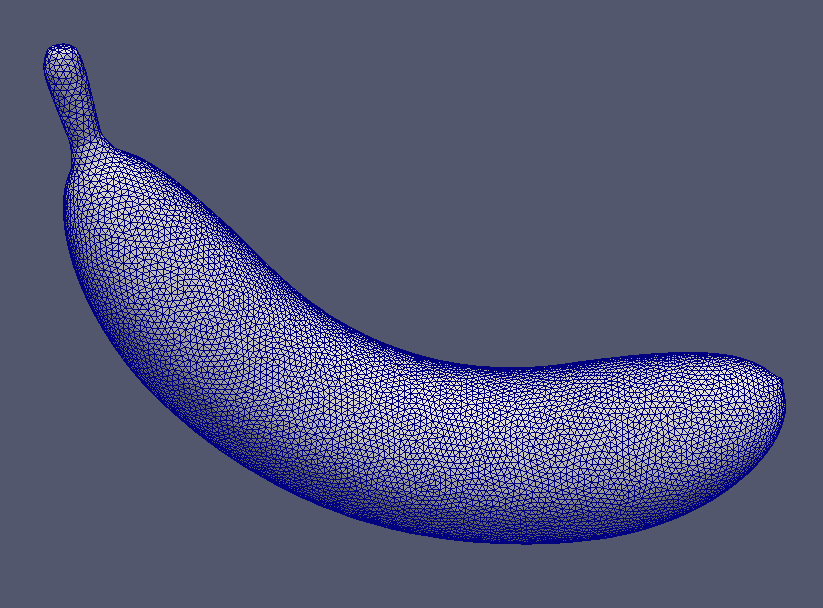
\includegraphics[width=\textwidth]{banana.png}
    \end{subfigure}
    \begin{subfigure}[b]{0.4\textwidth}
      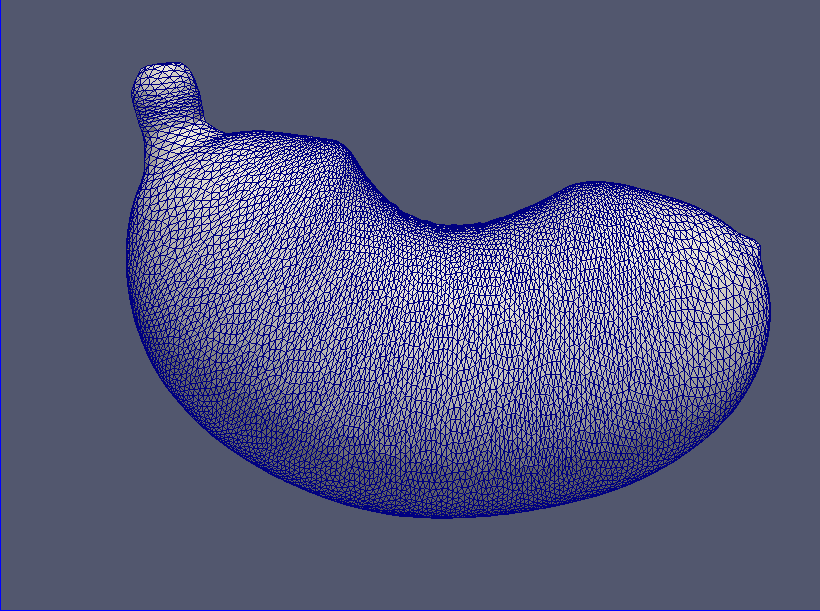
\includegraphics[width=\textwidth]{banana_deformed.png}
    \end{subfigure}
    \caption[banana形变结果]{原网格(a)和用我们的形变算法形变之后的网格(b)}
    \label{fig:banana-deform}
\end{figure}

\begin{figure}[htbp]
  \centering
  \begin{subfigure}[b]{0.4\textwidth}
    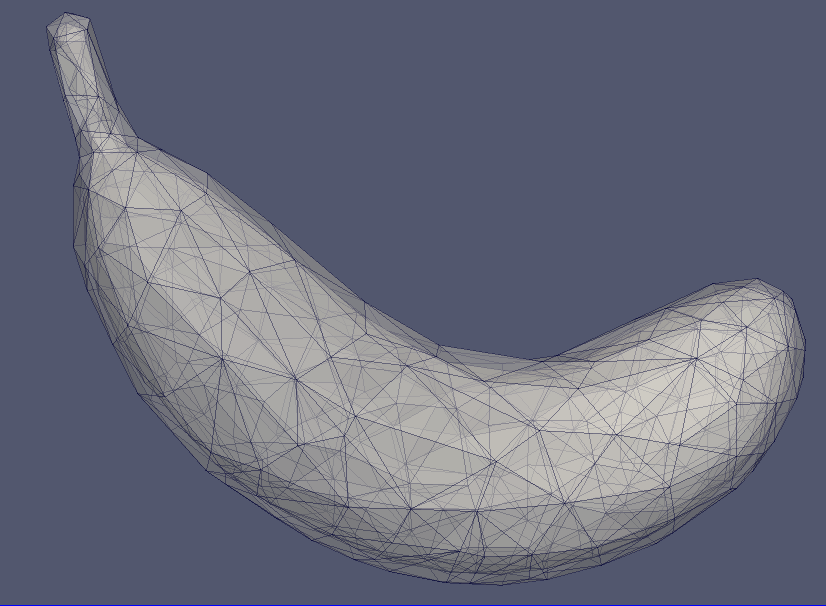
\includegraphics[width=\textwidth]{BANANA_0_0.06_0.03_0.12_100_refine.png}
  \end{subfigure}
  \begin{subfigure}[b]{0.4\textwidth}
    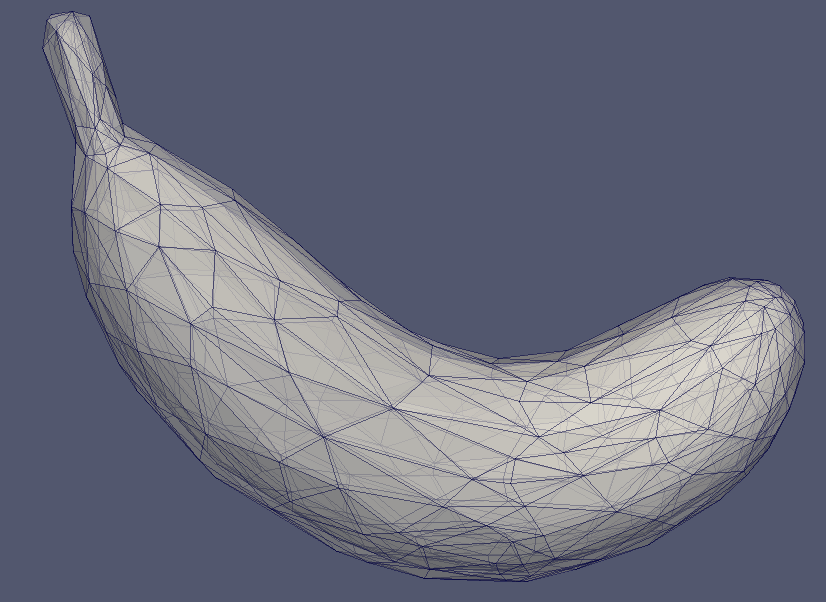
\includegraphics[width=\textwidth]{BANANA_1_0.06_0.03_0.12_100_refine.png}
  \end{subfigure}
  \begin{subfigure}[b]{0.4\textwidth}
    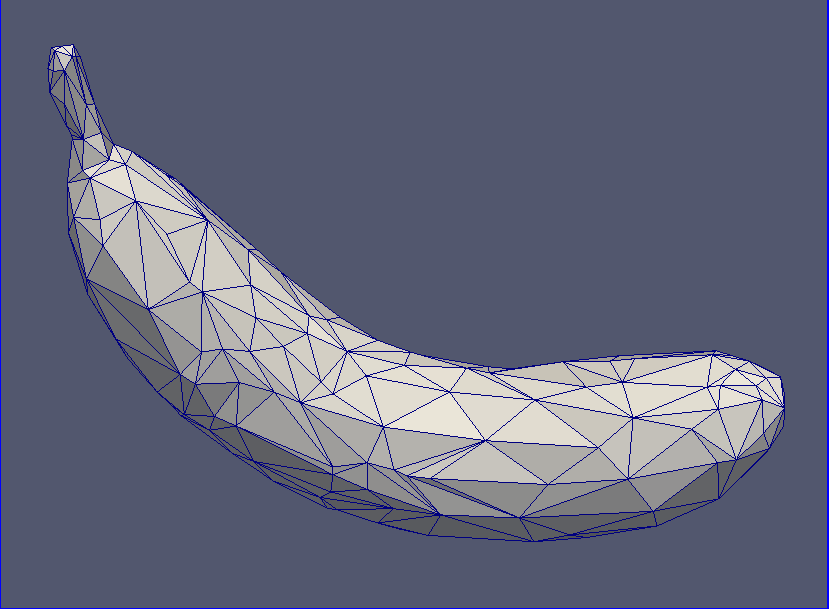
\includegraphics[width=\textwidth]{BANANA_0_0.06_0.03_0.12_100.png}
  \end{subfigure}
  \begin{subfigure}[b]{0.4\textwidth}
    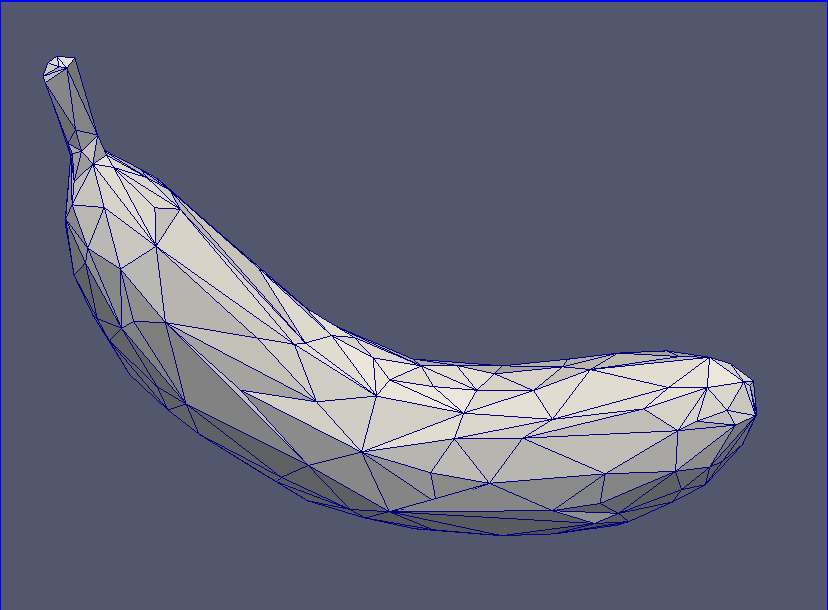
\includegraphics[width=\textwidth]{BANANA_1_0.06_0.03_0.12_100.png}
  \end{subfigure}
  \caption[当$\delta=0.5\%$时banana结果对比]{当$\delta=0.5\%$时,原算法的细化结果(左上图)和我们的算法的细化结果(右上图),原算法的简化结果(左下图,最终顶点数量为248)和我们的算法的简化结果(右下图,最终顶点数量为211)}
  \label{fig:banana-res1}
\end{figure}

\begin{figure}[htbp]
  \centering
  \begin{subfigure}[b]{0.4\textwidth}
    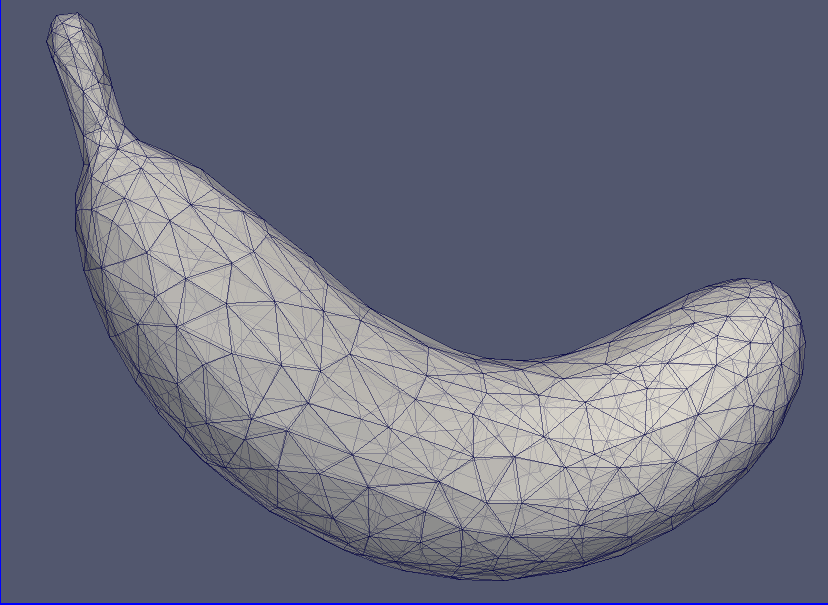
\includegraphics[width=\textwidth]{BANANA_0_0.03_0.015_0.06_100_refine.png}
  \end{subfigure}
  \begin{subfigure}[b]{0.4\textwidth}
    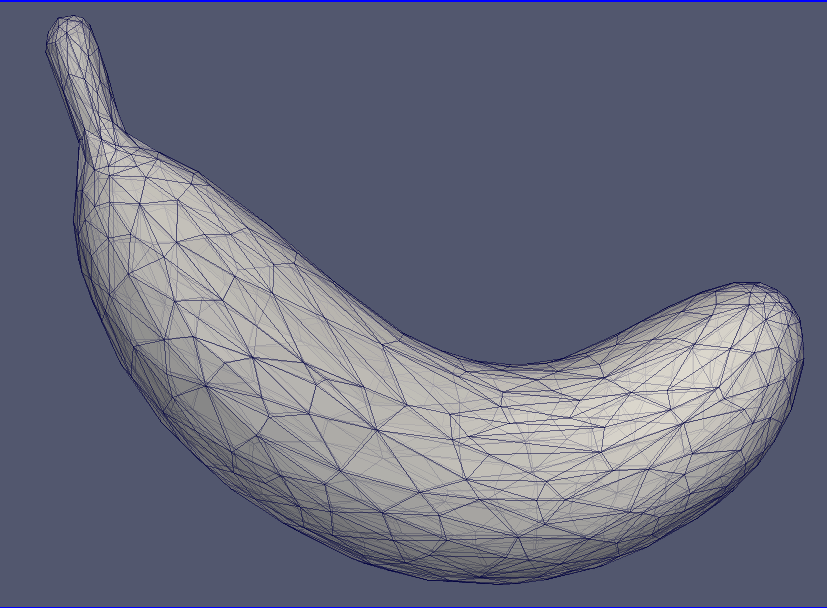
\includegraphics[width=\textwidth]{BANANA_1_0.03_0.015_0.06_100_refine.png}
  \end{subfigure}
  \begin{subfigure}[b]{0.4\textwidth}
    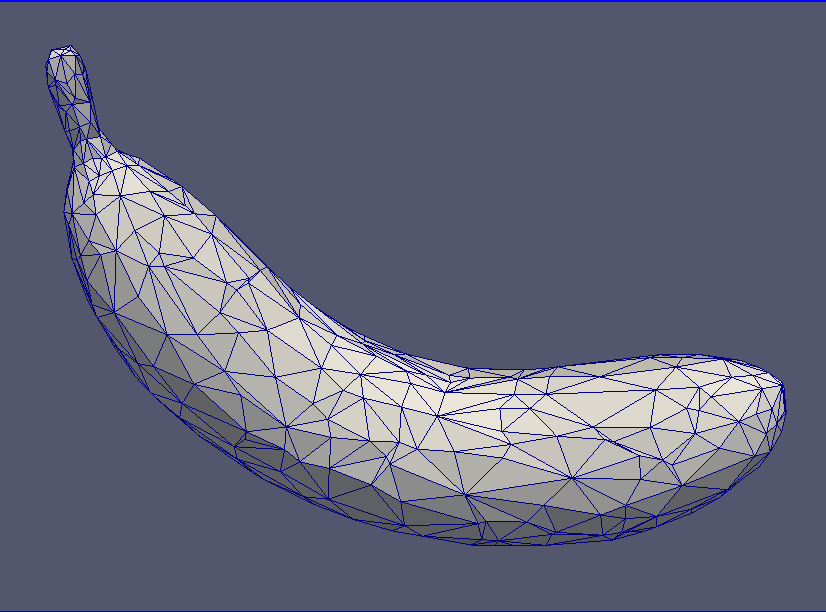
\includegraphics[width=\textwidth]{BANANA_0_0.03_0.015_0.06_100.png}
  \end{subfigure}
  \begin{subfigure}[b]{0.4\textwidth}
    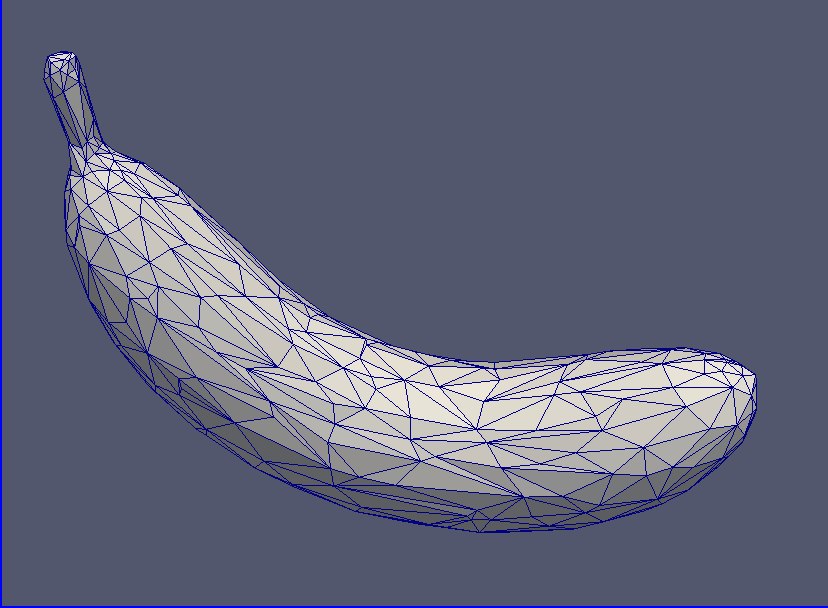
\includegraphics[width=\textwidth]{BANANA_1_0.03_0.015_0.06_100.png}
  \end{subfigure}
  \caption[当$\delta=0.25\%$时banana结果对比]{当$\delta=0.25\%$时,原算法的细化结果(左上图)和我们的算法的细化结果(右上图),原算法的简化结果(左下图,最终顶点数量为474)和我们的算法的简化结果(右下图,最终顶点数量为437)}
  \label{fig:banana-res2}
\end{figure}

\section{大白模型}
在大白模型(顶点数量为20000)上,我们的算法和原算法的结果对比:
\begin{figure}[htbp]
  \centering
  \begin{subfigure}[b]{0.4\textwidth}
    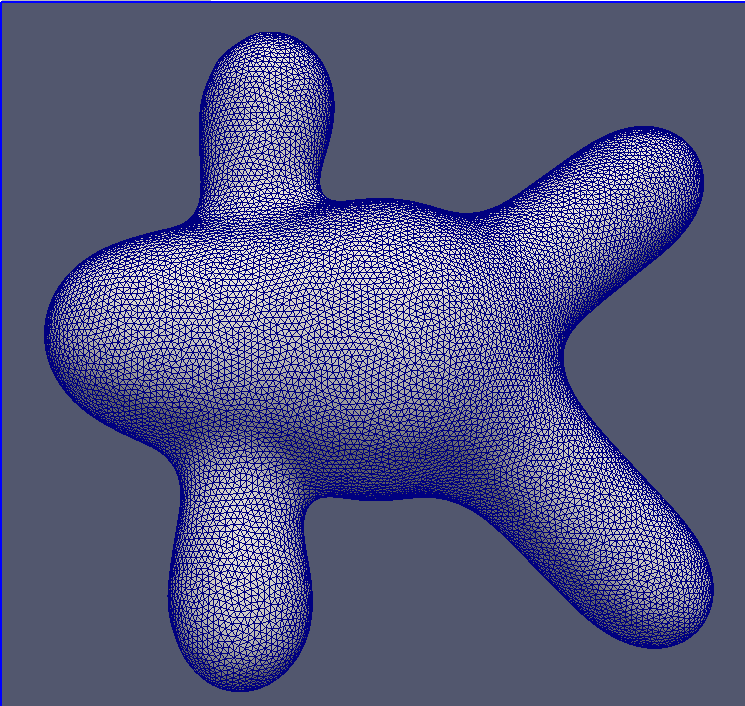
\includegraphics[width=\textwidth]{creature.png}
    \end{subfigure}
    \begin{subfigure}[b]{0.4\textwidth}
      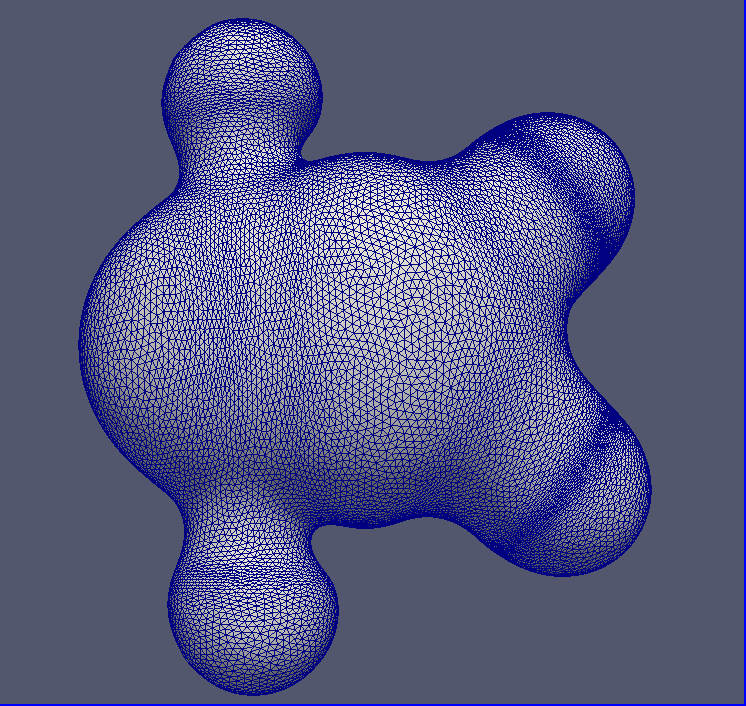
\includegraphics[width=\textwidth]{creature_deformed.png}
    \end{subfigure}
    \caption[大白的形变结果]{原网格(a)和用我们的形变算法形变之后的网格(b)}
    \label{fig:creature-deform}
\end{figure}

\begin{figure}[htbp]
  \centering
  \begin{subfigure}[b]{0.4\textwidth}
    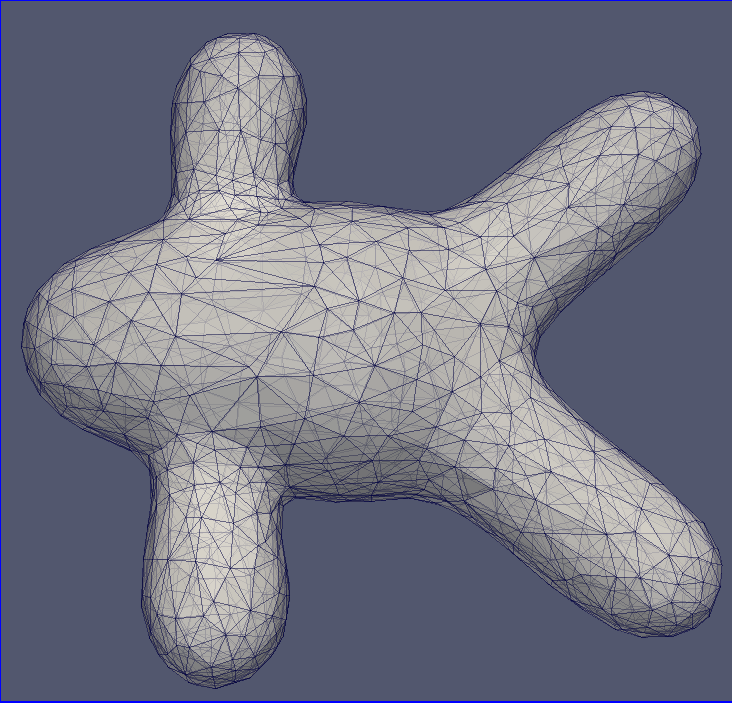
\includegraphics[width=\textwidth]{CREATURE_0_0.05_0.025_0.1_100_refine.png}
  \end{subfigure}
  \begin{subfigure}[b]{0.4\textwidth}
    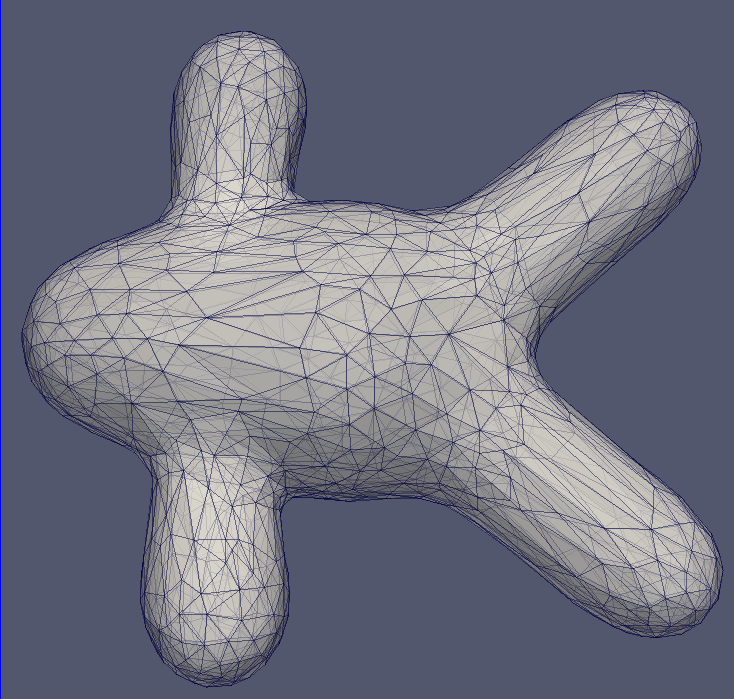
\includegraphics[width=\textwidth]{CREATURE_1_0.05_0.025_0.1_100_refine.png}
  \end{subfigure}
  \begin{subfigure}[b]{0.4\textwidth}
    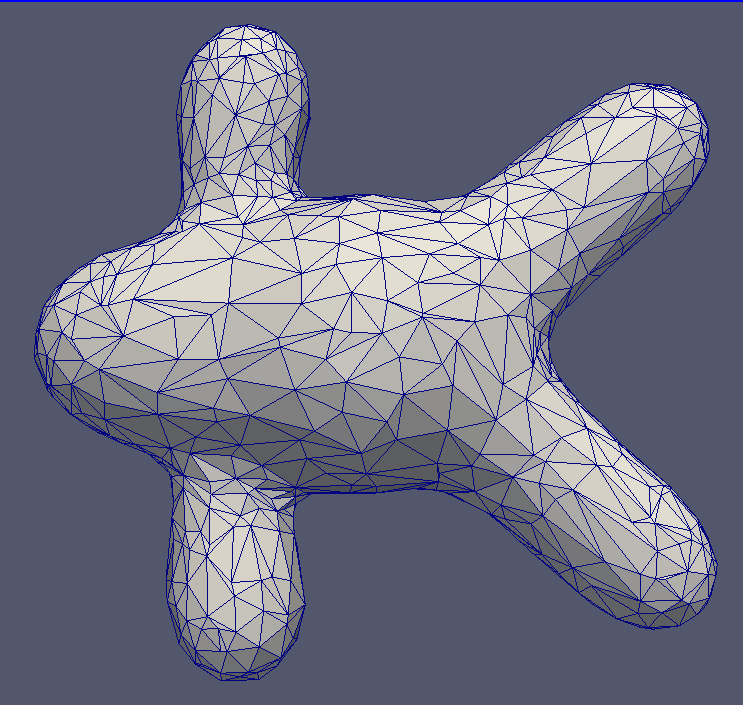
\includegraphics[width=\textwidth]{CREATURE_0_0.05_0.025_0.1_100.png}
  \end{subfigure}
  \begin{subfigure}[b]{0.4\textwidth}
    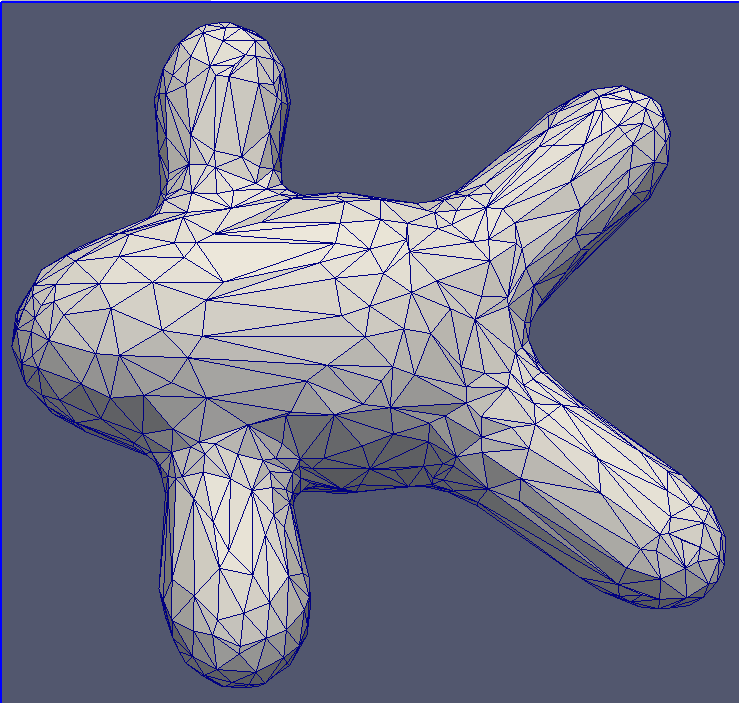
\includegraphics[width=\textwidth]{CREATURE_1_0.05_0.025_0.1_100.png}
  \end{subfigure}
  \caption[当$\delta=0.22\%$时banana结果对比]{当$\delta=0.22\%$时,原算法的细化结果(左上图)和我们的算法的细化结果(右上图),原算法的简化结果(左下图,最终顶点数量为958)和我们的算法的简化结果(右下图,最终顶点数量为852)}
  \label{fig:creature-res1}
\end{figure}

\begin{figure}[htbp]
  \centering
  \begin{subfigure}[b]{0.4\textwidth}
    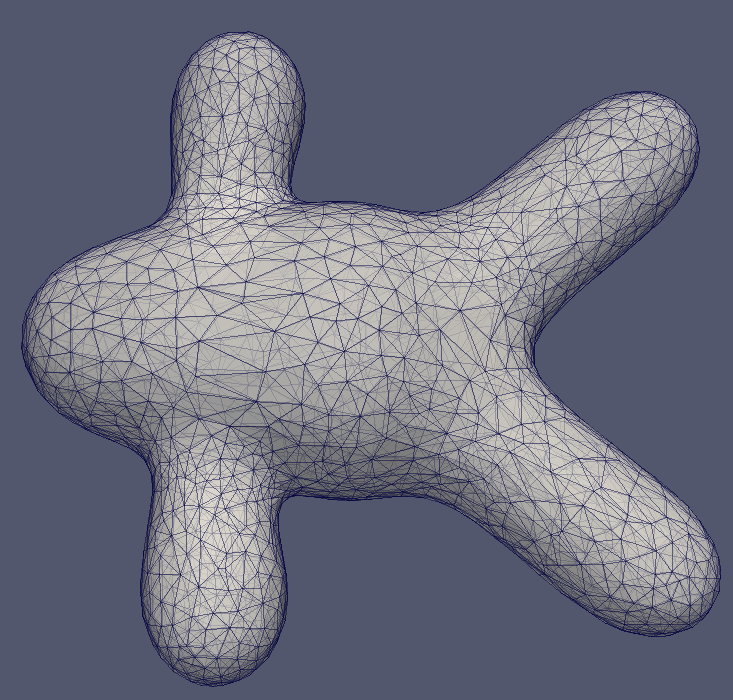
\includegraphics[width=\textwidth]{CREATURE_0_0.025_0.015_0.05_100_refine.png}
  \end{subfigure}
  \begin{subfigure}[b]{0.4\textwidth}
    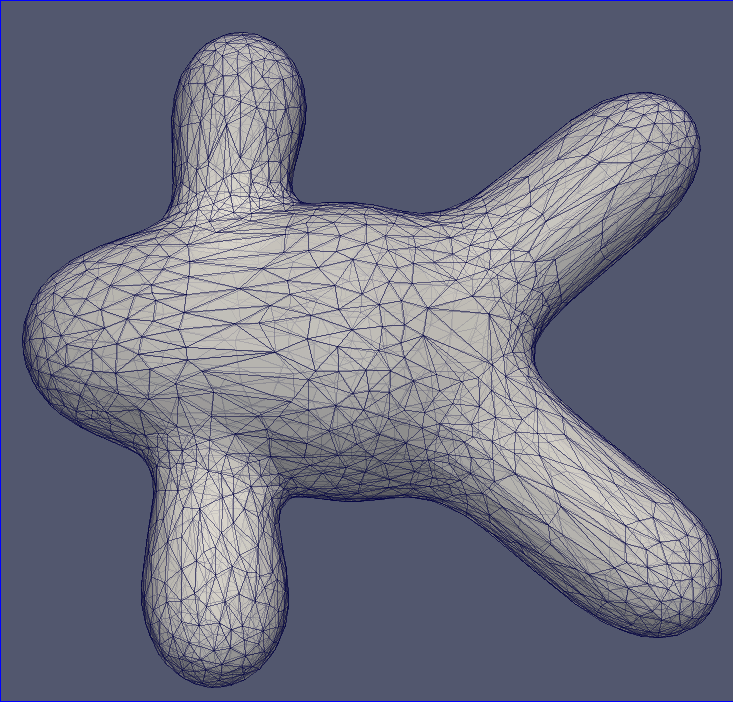
\includegraphics[width=\textwidth]{CREATURE_1_0.025_0.015_0.05_100_refine.png}
  \end{subfigure}
  \begin{subfigure}[b]{0.4\textwidth}
    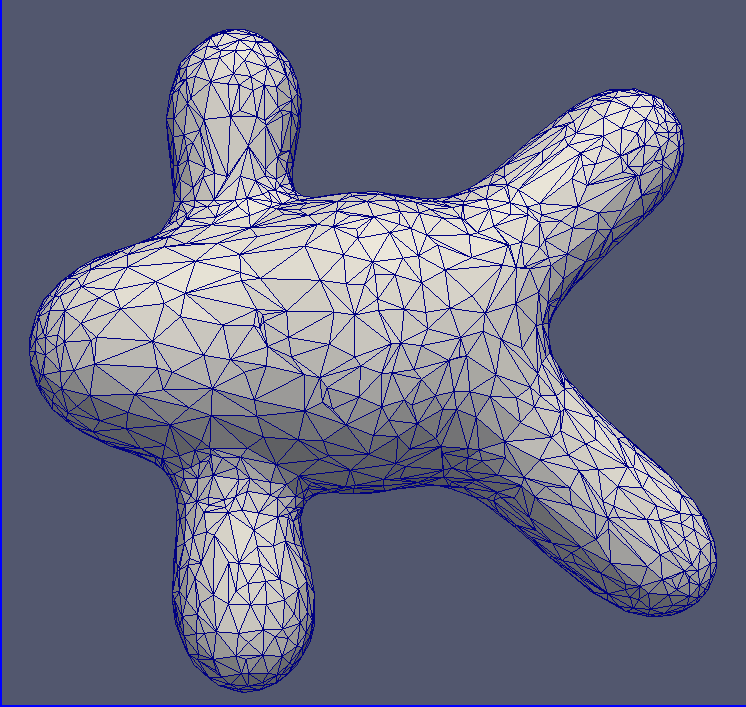
\includegraphics[width=\textwidth]{CREATURE_0_0.025_0.015_0.05_100.png}
  \end{subfigure}
  \begin{subfigure}[b]{0.4\textwidth}
    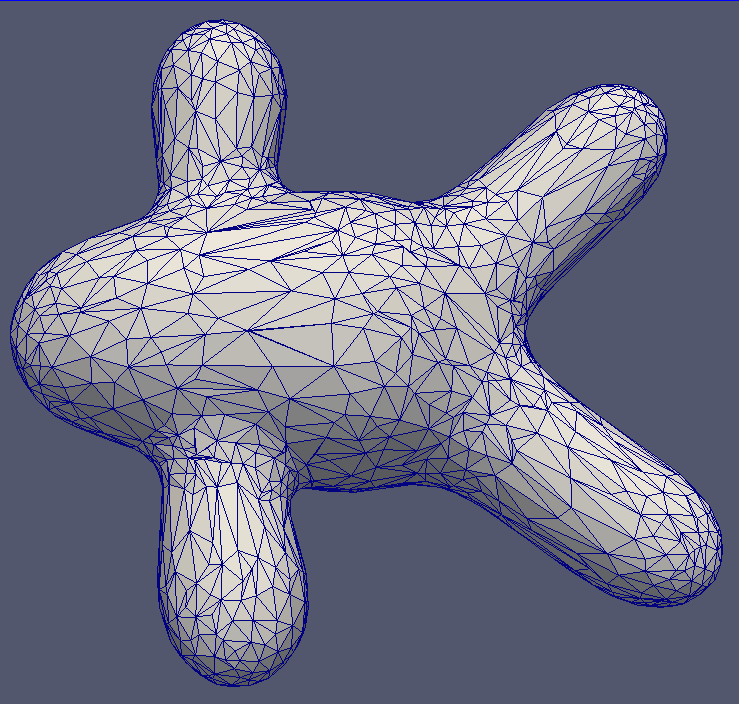
\includegraphics[width=\textwidth]{CREATURE_1_0.025_0.015_0.05_100.png}
  \end{subfigure}
  \caption[当$\delta=0.11\%$时banana结果对比]{当$\delta=0.11\%$时,原算法的细化结果(左上图)和我们的算法的细化结果(右上图),原算法的简化结果(左下图,最终顶点数量为1911)和我们的算法的简化结果(右下图,最终顶点数量为1725)}
  \label{fig:creature-res2}
\end{figure}

\section{Fertility模型}
在Fertility模型(顶点数量为1397)上与原算法的结果对比:
\begin{figure}[htbp]
  \centering
  \begin{subfigure}[b]{0.4\textwidth}
    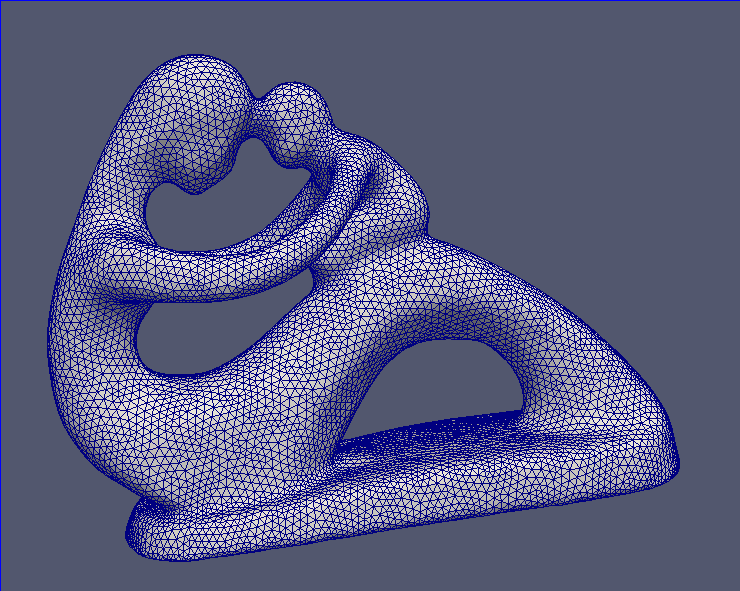
\includegraphics[width=\textwidth]{fertility.png}
    \end{subfigure}
    \begin{subfigure}[b]{0.4\textwidth}
      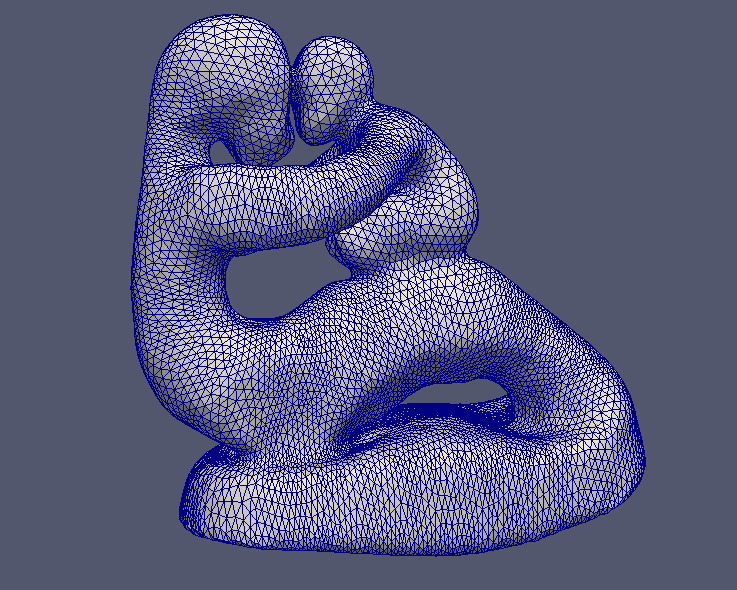
\includegraphics[width=\textwidth]{fertility_deformed.png}
    \end{subfigure}
    \caption[fertility形变结果]{原网格(a)和用我们的形变算法形变之后的网格(b)}
    \label{fig:fertility-deform}
\end{figure}

\begin{figure}[htbp]
  \centering
  \begin{subfigure}[b]{0.4\textwidth}
    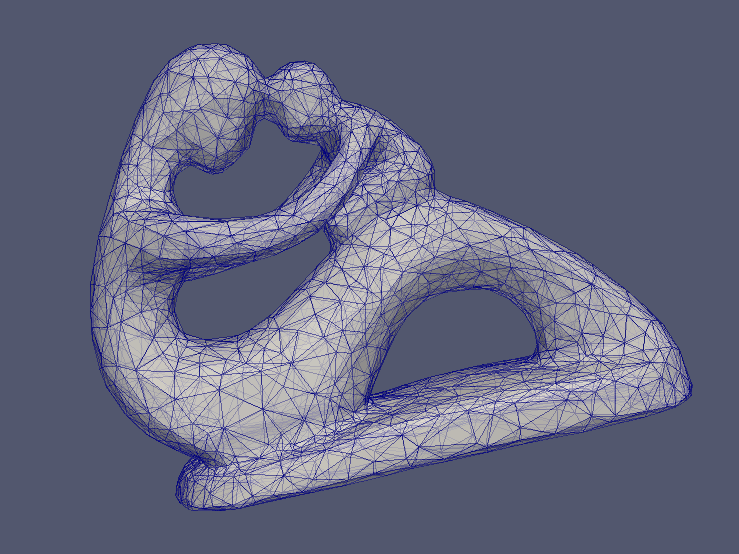
\includegraphics[width=\textwidth]{FERTILITY_0_0.5_0.25_1.5_100_refine.png}
  \end{subfigure}
  \begin{subfigure}[b]{0.4\textwidth}
    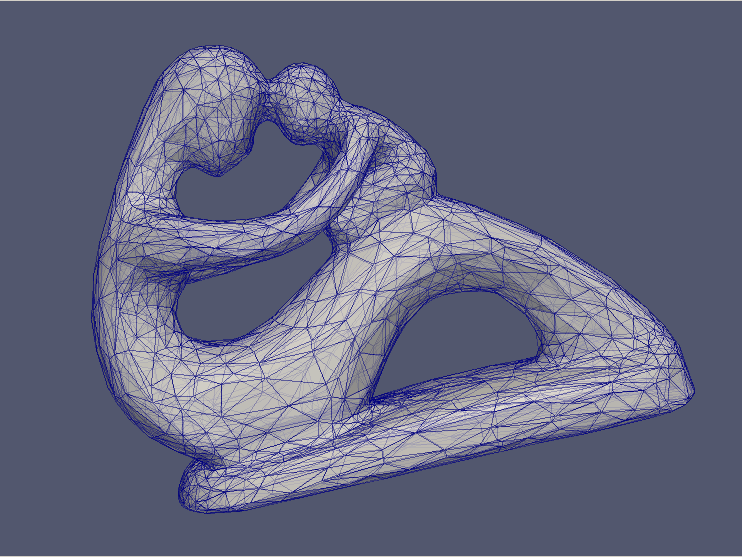
\includegraphics[width=\textwidth]{FERTILITY_1_0.5_0.25_1.5_100_refine.png}
  \end{subfigure}
  \begin{subfigure}[b]{0.4\textwidth}
    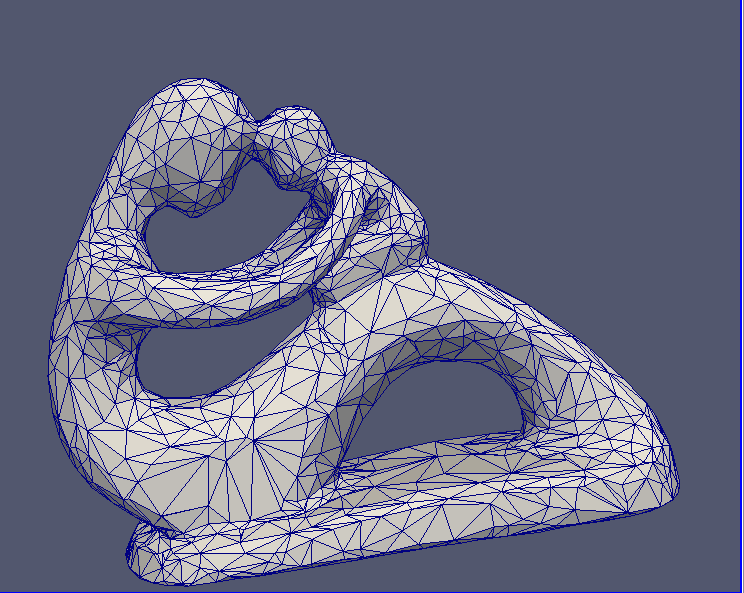
\includegraphics[width=\textwidth]{FERTILITY_0_0.5_0.25_1.5_100.png}
  \end{subfigure}
  \begin{subfigure}[b]{0.4\textwidth}
    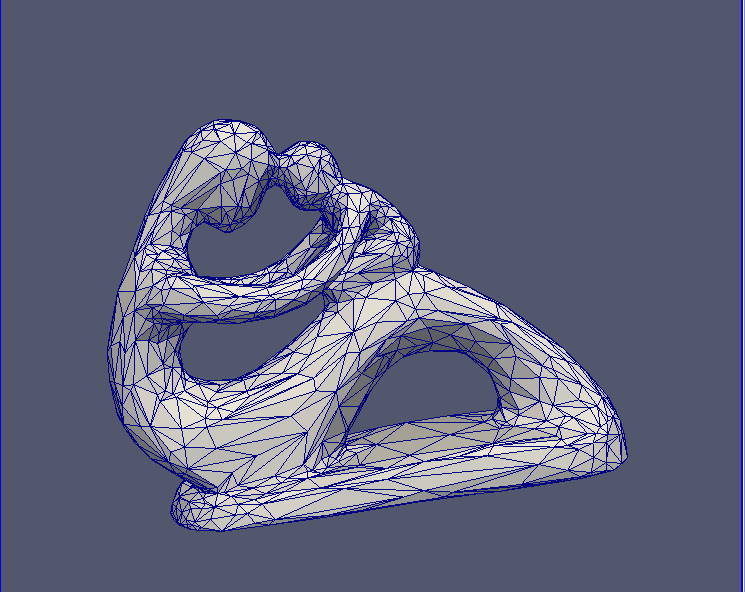
\includegraphics[width=\textwidth]{FERTILITY_1_0.5_0.25_1.5_100.png}
  \end{subfigure}
  \caption[当$\delta=0.1948\%$时fertility结果对比]{当$\delta=0.1948\%$时,原算法的细化结果(左上图)和我们的算法的细化结果(右上图),原算法的简化结果(左下图,最终顶点数量为1784)和我们的算法的简化结果(右下图,最终顶点数量为1640)}
  \label{fig:fertility-res1}
\end{figure}

\begin{figure}[htbp]
  \centering
  \begin{subfigure}[b]{0.4\textwidth}
    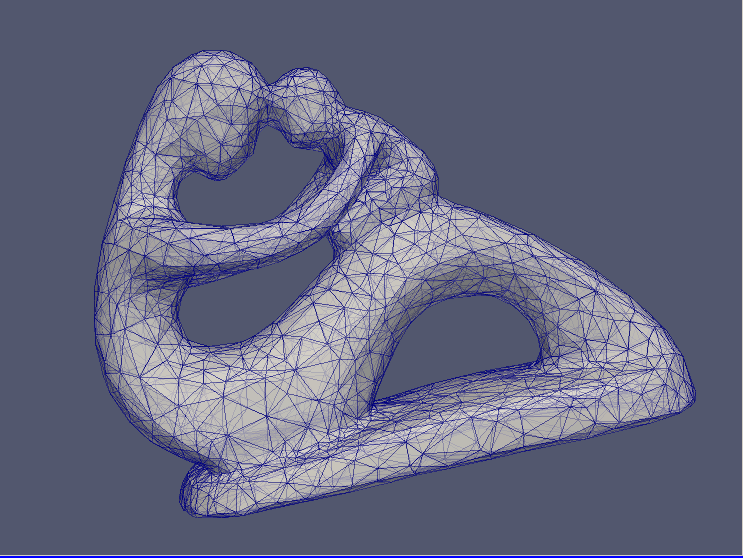
\includegraphics[width=\textwidth]{FERTILITY_0_0.25_0.125_1_100_refine.png}
  \end{subfigure}
  \begin{subfigure}[b]{0.4\textwidth}
    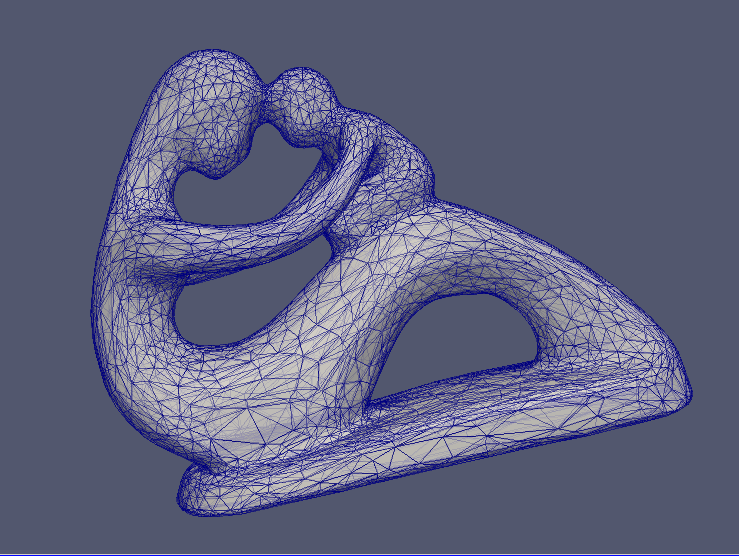
\includegraphics[width=\textwidth]{FERTILITY_1_0.25_0.125_1_100_refine.png}
  \end{subfigure}
  \begin{subfigure}[b]{0.4\textwidth}
    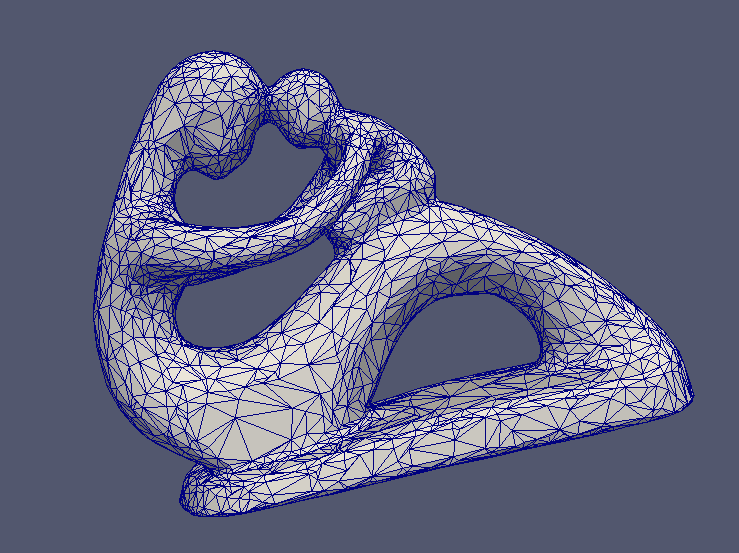
\includegraphics[width=\textwidth]{FERTILITY_0_0.25_0.125_1_100.png}
  \end{subfigure}
  \begin{subfigure}[b]{0.4\textwidth}
    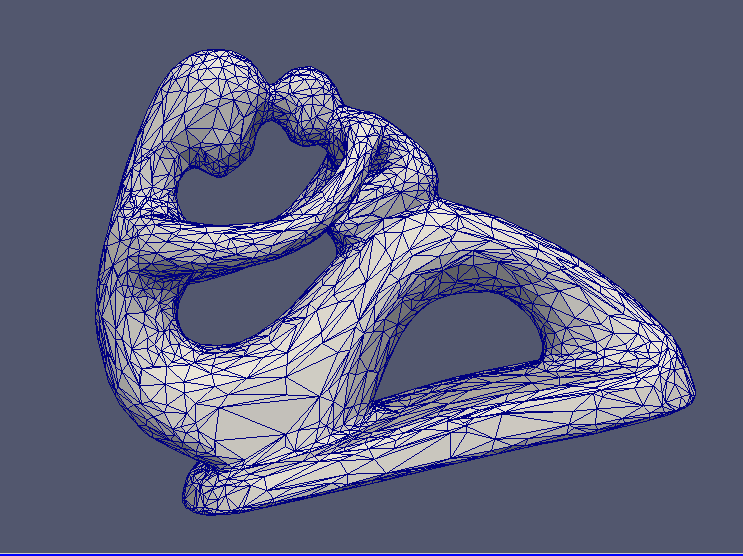
\includegraphics[width=\textwidth]{FERTILITY_1_0.25_0.125_1_100.png}
  \end{subfigure}
  \caption[当$\delta=0.0974\%$时fertility结果对比]{当$\delta=0.0974\%$时,原算法的细化结果(左上图)和我们的算法的细化结果(右上图),原算法的简化结果(左下图,最终顶点数量为3832)和我们的算法的简化结果(右下图,最终顶点数量为3550)}
  \label{fig:fertility-res2}
\end{figure}
